% ----------------------------------------------------------
\chapter{Desenvolvimento do Projeto}
% ----------------------------------------------------------

Após estudar os desdobramentos dos efeitos de órbita baixa e entender o que é necessário para se realizar um projeto confiável de computador de bordo de um nanossatélite, foi necessária a compreensão dos pré-requisitos de projeto. Com isso, foram escolhidos os componentes principais da placa, e a partir deles, um esquemático elétrico foi construído, propondo enfim um hardware confiável, robusto e versátil.  

\section{Pré-Requisitos de Projeto}

Como dito, foi preciso entender os pré-requisitos impostos para o OBDH da terceira geração do SpaceLab. Abaixo, na Tabela \ref{tab:Tab_Req}, se encontram os requisitos gerais do projeto, em conjunto com o pretexto e com o nível de prioridade.

\begin{longtable}{@{}p{5cm}p{5cm}p{3.5cm}@{}}
    \centering
	\ABNTEXfontereduzida
	\label{tab:Tab_Req}\tabularnewline
	\caption{Requisitos do projeto.}\tabularnewline
	%\begin{tabular}{@{}p{2cm}p{2cm}p{2cm}p{2cm}p{2cm}p{2cm}p{3cm}@{}}
	\hline
	\textbf{\centering{Descrição}} & \textbf{\centering{Pretexto}} & \textbf{\centering{Prioridade}} \tabularnewline
        \hline
        O módulo OBDH deve ser compatível com o padrão CubeSat & Assegura compatibilidade com outros satélites desenvolvidos no SpaceLab & Alta \tabularnewline
        
       \hline
        O módulo OBDH deve operar corretamente entre -40°C e 85°C & Para operar com segurança em um ambiente LEO & Alta \tabularnewline

       \hline
        O módulo OBDH deve possuir um microcontrolador capaz de usar um sistema Linux & Para gerenciar e coordenar operações dentro e fora do módulo, sendo capaz de realizar tarefas complexas  & Alta \tabularnewline

       \hline
        O módulo OBDH deve possuir uma memória DDR com capacidade de 512Mb (preferencialmente com ECC)  & Memória suficiente para operações do OBDH e armazenamento de dados  & Alta\tabularnewline

        \hline
        O módulo OBDH deve possuir uma memória FRAM para armazenar parâmetros de configuração & Provê memória não-volátil e duradoura, menos sucetível à radiação & Alta \tabularnewline 

        \hline
        O módulo OBDH deve possuir uma memória Flash para armazenar pacotes (preferencialmente com ECC) & Para armazenar dados e pacotes recebidos & Alta\tabularnewline 

        \hline
        O módulo OBDH deve possuir um WDT para reiniciar o microcontrolador em caso de falha de \textit{software} & Reinicia automaticamente o microcontrolador caso haja a falha  & Alta \tabularnewline

        \hline
        O módulo OBDH deve possuir sensores de medição de tensão e corrente em suas tensões & Para monitoramento de potência consumida & Alta\tabularnewline

        \hline
        O módulo OBDH deve possuir proteção de sobrecorrente (20\% acima do valor nominal) & Para proteção contra \textit{latch-up}  & Alta \tabularnewline

        \hline
        O módulo OBDH deve possuir um giroscópio para medição de velocidade angular & Para permitir controle ativo do satélite  & Alta \tabularnewline 

       \hline
        O módulo OBDH deve possuir um magnetômetro & Para permitir controle ativo do satélite  & Alta \tabularnewline

        \hline
        O módulo OBDH deve possuir uma interface RS-422 para transmissão de mensagens de \textit{debug/log} e receber parâmetros de configuração & Comunicação de longa distância com maior imunidade ao ruído e maior taxa de dados (comparando com UART)  & Alta \tabularnewline

       \hline
        O módulo OBDH deve possuir uma interface CAN para receber e transmitir comandos e dados & Comunicação robusta e com suporte a múltiplos sistemas do CubeSat  & Alta\tabularnewline

        \hline
        O módulo OBDH deve possuir uma interface acessível externamente para programação do microcontrolador & Para o módulo ser facilmente programado pelo time  & Alta \tabularnewline

        \hline
        O módulo OBDH deve possuir uma interface para uma \textit{daughter board} & Para prover suporte a outras interfaces e periféricos  & Baixa \tabularnewline

        \hline
        O módulo OBDH deve possuir um sensor de temperatura com precisão menor ou igual a 1°C & Para prevenir danos de temperaturas extremas & Baixa\tabularnewline

        \hline
        O módulo OBDH deve possuir uma interface RS-485 para receber e transmitir comandos e dados  & Para transmissão robusta de dados com módulos externos & Baixa \tabularnewline
       \hline
	\centering{\fonte{Elaboração própria.}}
\end{longtable}

Com as definições apresentadas na Tabela \ref{tab:Tab_Req}, foi então necessária a definição da arquitetura do hardware, ou seja, os componentes e sua interconexões, bem como as interfaces de comunicação e saídas necessárias.

\section{Arquitetura}

A partir dos requisitos, o primeiro passo foi definir de forma geral como seria o funcionamento do \textit{hardware} do projeto. Na Figura \ref{fig:arq_geral}, pode-se verificar um esquema inicial de proposta de arquitetura, usando os pontos descritos anteriormente.

\begin{figure}[htp]
    \centering
    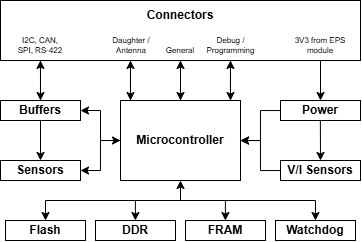
\includegraphics[scale=0.7]{images/arquitetura geral.png}
    \caption{Arquitetura proposta.}
    \label{fig:arq_geral}
\end{figure}

Como podemos verificar, o microprocessador será crucial e deverá ter pinos suficientes para interface com todas as memórias, sensores e para se comunicar com os outros módulos do CubeSat. Além disso, a parte dedicada às tensões usadas deverá ser cuidadosamente feita, para suportar a potência dissipada por todos os componentes da placa de circuito impresso. A escolha de cada componente será descrita nas seções a seguir, respeitando sempre os seguintes critérios:

\begin{itemize}
	\item O componente deve funcionar corretamente nas temperaturas entre -40°C e 85°C;
	\item Circuitos integrados devem possuir herança de voo sempre que possível;
	\item Caso o circuito integrado necessite de um circuito específico, o mesmo deve conter itens preferencialmente dispostos na ECSS-Q-ST-60C, na NPSL ou similar aos mesmos, especialmente componentes discretos (capacitores, resistores, indutores, diodos, transistores, entre outros);
\end{itemize}

\subsection{Microcontrolador}

Como visto na Tabela \ref{tab:Tab_Missoes}, a fabricante com maior herança de voo estudada é a Xilinx, em especial os chips da família Zynq 7000, que são SoCs (\textit{System on a Chip}). Após um estudo próprio, o SoC Zynq 7030 se mostrou mais adequado pelas seguintes características:

\begin{itemize}
	\item Foi usado em missões extensivas em pequenos satélites (Gomspace, 2024), ou seja, possui herança de voo em missões similares em LEO e em CubeSats;
	\item Possui um envelopamento com 484 pinos, suficiente para prover as conexões necessárias para todas as interfaces requeridas (UG865, 2021);
	\item Capaz de rodar um sistema Linux (KADI et al.,2013);
	\item Por ser um SoC, possui alta adaptabilidade e flexibilidade, disponibilizando no mesmo chip uma FPGA (PL, \textit{Programmable Logic}) e um microprocessador (PS, \textit{Processing System});
\end{itemize}

\subsection{Memórias}

As memórias serão necessárias para realizar operações, armazenar dados externos e internos e armazenar parâmetros de configuração do OBDH e de outros subsistemas do CubeSat. Para cada uma dessas funções uma memória diferente é necessária, seguindo suas características principais, sendo elas: tempo de acesso, tamanho do armazenamento e volatilidade.

\subsubsection{Memórias voláteis}




